%
% Niniejszy plik stanowi przykład formatowania pracy magisterskiej na
% Wydziale MIM UW.  Szkielet użytych poleceń można wykorzystywać do
% woli, np. formatujac wlasna prace.
%
% Zawartosc merytoryczna stanowi oryginalnosiagniecie
% naukowosciowe Marcina Wolinskiego.  Wszelkie prawa zastrzeżone.
%
% Copyright (c) 2001 by Marcin Woliński <M.Wolinski@gust.org.pl>
% Poprawki spowodowane zmianami przepisów - Marcin Szczuka, 1.10.2004
% Poprawki spowodowane zmianami przepisow i ujednolicenie 
% - Seweryn Karłowicz, 05.05.2006
% Dodanie wielu autorów i tłumaczenia na angielski - Kuba Pochrybniak, 29.11.2016

% dodaj opcję [licencjacka] dla pracy licencjackiej
% dodaj opcję [en] dla wersji angielskiej (mogą być obie: [licencjacka,en])

\documentclass[licencjacka]{pracamgr}

\usepackage{graphicx}
\usepackage{placeins}

% Dane magistranta:
% \autor{Imię Nazwisko}{123456}


% Dane magistrantów:
\autor{Antoni Rajtar}{448467}
\autori{Jacek Kajdan}{448273}

\autorii{Dawid Ratyński}{448571}
\autoriii{Aleksandra Wolska}{431567}
%\autoriv{Dawid Ratyński}{448571}
%\autorv{Aleksandra Wolska}{431567}

\title{CleanTheWorld (tytuł roboczy)}


%\tytulang{An implementation of a difference blabalizer based on the theory of $\sigma$ -- $\rho$ phetors}

%kierunek: 
% - matematyka, informacyka, ...
% - Mathematics, Computer Science, ...
\kierunek{informatyka}

% informatyka - nie okreslamy zakresu (opcja zakomentowana)
% matematyka - zakres moze pozostac nieokreslony,
% a jesli ma byc okreslony dla pracy mgr,
% to przyjmuje jedna z wartosci:
% {metod matematycznych w finansach}
% {metod matematycznych w ubezpieczeniach}
% {matematyki stosowanej}
% {nauczania matematyki}
% Dla pracy licencjackiej mamy natomiast
% mozliwosc wpisania takiej wartosci zakresu:
% {Jednoczesnych Studiow Ekonomiczno--Matematycznych}

% \zakres{Tu wpisac, jesli trzeba, jedna z opcji podanych wyzej}

% Praca wykonana pod kierunkiem:
% (podać tytuł/stopień imię i nazwisko opiekuna
% Instytut
% ew. Wydział ew. Uczelnia (jeżeli nie MIM UW))
\opiekun{mgr. Krzysztof Ciebiera\\
  Instytut Informatyki\\
  }

% miesiąc i~rok:
\date{Maj 2025}

%Podać dziedzinę wg klasyfikacji Socrates-Erasmus:
\dziedzina{ 
%11.0 Matematyka, Informatyka:\\ 
%11.1 Matematyka\\ 
%11.2 Statystyka\\ 
11.3 Informatyka\\ 
11.4 Sztuczna inteligencja\\ 
%11.5 Nauki aktuarialne\\
%11.9 Inne nauki matematyczne i informatyczne
}

%Klasyfikacja tematyczna wedlug AMS (matematyka) lub ACM (informatyka)

\klasyfikacja{TODO}

% Słowa kluczowe:
\keywords{TODO}

\tytulang{TODO}
% Tu jest dobre miejsce na Twoje własne makra i~środowiska:
\newtheorem{defi}{Definicja}[section]

% koniec definicji

\begin{document}

\maketitle

%tu idzie streszczenie na strone poczatkowa
\begin{abstract}
% W~pracy przedstawiono prototypową implementację blabalizatora
% różnicowego bazującą na teorii fetorów $\sigma$-$\rho$ profesora
% Fifaka.  Wykorzystanie teorii Fifaka daje wreszcie możliwość
% efektywnego wykonania blabalizy numerycznej.  Fakt ten stanowi
% przełom technologiczny, którego konsekwencje trudno z~góry
% przewidzieć.
TODO
\end{abstract}

\tableofcontents
%\listoffigures
%\listoftables

\chapter*{Wprowadzenie}
\addcontentsline{toc}{chapter}{Wprowadzenie}

% Blabalizator różnicowy jest podstawowym narzędziem blabalii
% fetorycznej.  Dlatego naukowcy z~całego świata prześcigają się
% w~próbach efektywnej implementacji.  Opracowana przez prof. Fifaka
% teoria fetorów $\sigma$-$\rho$ otwiera w~tej dziedzinie nowe
% możliwości.  Wykorzystujemy je w~niniejszej pracy.
% 
% Przystępne wprowadzenie do blabalii fetorycznej można znaleźć w~pracy
% Fifaka i~Gryzogrzechotalskiego \cite{ffgg}.  Dlatego w~niniejszym
% tekście ograniczymy się do przypomnienia pojęć podstawowych.
% 
% Praca składa się z~pięciu rozdziałów i~dodatków.
% W~rozdziale~\ref{r:pojecia} przypomniano podstawowe pojęcia blabalii
% fetorycznej.  Dotychczasowe próby implementacji blablizatora
% różnicowego zestawiono w~rozdziale~\ref{r:losers}.
% Rozdział~\ref{r:fifak} przedstawia teorię Fifaka i~wyjaśnia sposób jej
% wykorzystania w~implementacji blabalizatora.  W~rozdziale \ref{r:impl}
% przedstawiono algorytm blabalizy i~realizujący go program komputerowy.
% Ostatni rozdział zawiera przemyślenia dotyczące możliwego wpływu
% dostępności efektywnej blabalizy numerycznej na rozwój blabalii
% fetorycznej.  W~dodatkach umieszczono najciekawszy fragment programu,
% przykładowe dane i~wyniki działania programu.
TODO

\chapter{Podstawowe pojęcia}\label{r:pojecia}

%Pojęciem pierwotnym blabalii fetorycznej jest \emph{blaba}.
%Blabaliści nie podają jego definicji, mówiąc za Ciach-Pfe t-\=am
%K\^un (fooistyczny mędrzec, XIX w. p.n.e.):
%\begin{quote}
%  Blaba, który jest blaba, nie jest prawdziwym blaba.

%\raggedleft\slshape tłum. z~chińskiego Robert Blarbarucki
%\end{quote}

%Pojęciem kluczowym w dziedzinie analizy obrazów jest obiekt (ang. \emph{bounding box}).
%Podobnie jak w klasycznej teorii rozpoznawania wzorców, obiekt definiowany jest jako spójny fragment obrazu, który może zostać przypisany do jednej z predefiniowanych kategorii. W kontekście niniejszej pracy obiektami są odpady.

\section{Definicje}

W analizie obrazu można wyróżnić trzy podstawowe zadania: detekcję, segmentację i klasyfikację, które pozwalają na identyfikację oraz interpretację zawartości obrazu.

\begin{defi}\label{detekcja}
    \emph{Detekcja obiektów} polega na lokalizowaniu i klasyfikowaniu obiektów w obrazie lub wideo.
\end{defi}

Aby umożliwić identyfikację obiektów, w zadaniach detekcji obiektów stosuje się \textbf{ramki ograniczające} (\emph{bounding boxes}), które określają prostokątny obszar na obrazie zawierający dany obiekt. Ramki te są wykorzystywane zarówno podczas trenowania modeli, jak i w trakcie predykcji, umożliwiając lokalizację obiektów w przestrzeni obrazu. Poprawność wykrycia obiektu zależy nie tylko od prawidłowego przypisania klasy, ale także od precyzyjnego umiejscowienia ramki. 

\begin{defi}\label{seg}
    \emph{Segmentacja} to proces podziału obrazu lub wideo na interesujące regiony w celu identyfikacji i rozróżnienia obiektów lub regionów zainteresowania.
\end{defi}

\begin{defi}\label{segmentacja}
    \emph{Segmentacja semantyczna} polega na przypisaniu każdemu pikselowi w obrazie etykiety klasy, do której należy.
\end{defi}

\begin{defi}\label{klasyfikacja}
    \emph{Klasyfikacja} polega na przypisaniu całemu obrazowi jednej etykiety klasy spośród zbioru zdefiniowanych kategorii. Jest to podstawowe zadanie w rozpoznawaniu obrazów, które nie uwzględnia lokalizacji ani kształtu obiektów, a jedynie określa ich obecność.
\end{defi}

\section{Metryki oceny jakości}

\begin{defi}\label{iou}
\emph{Intersection over Union} (IoU) to metryka do mierzenia dokładności lokalizacji i obliczania błędów lokalizacji w modelach detekcji obiektów. Oblicza ona stopień nakładania się dwóch ramek ograniczających – przewidywanej ramki oraz rzeczywistej ramki.

\begin{equation}
IoU = \frac{|A \cap B|}{|A \cup B|}
\end{equation}

gdzie $A$ oznacza rzeczywistą (ground truth) maskę obiektu, a $B$ przewidywaną maskę wygenerowaną przez model. Wartość IoU mieści się w przedziale $[0,1]$, gdzie 1 oznacza idealne dopasowanie.
\end{defi}

Przy ocenie jakości klasyfikacji obiektów w systemach detekcji stosuje się kilka kluczowych pojęć, które opisują poprawność i błędy klasyfikacyjne. W szczególności wyróżnia się następujące kategorie wyników:

\begin{defi}\label{true_positive}
\emph{True Positive (TP)} – liczba obiektów poprawnie wykrytych jako należące do danej klasy. (prawdziwe pozytywy)
\end{defi}

\begin{defi}\label{false_positive}
\emph{False Positive (FP)} – liczba obiektów błędnie sklasyfikowanych jako należące do danej klasy (fałszywe pozytywy).
\end{defi}

\begin{defi}\label{false_negative}
\emph{False Negative (FN)} – liczba obiektów błędnie sklasyfikowanych jako nienależące do danej klasy (fałszywe negatywy).
\end{defi}

Na podstawie powyższych wartości definiuje się dwie kluczowe miary oceny skuteczności detekcji:

\begin{defi}\label{precision}
\emph{Precision} (precyzja) określa stosunek liczby poprawnie wykrytych obiektów (TP) do liczby wszystkich pozytywnych wykryć (TP + FP). Jest miarą jakości detekcji, eliminującą fałszywe pozytywy:

\begin{equation}
\text{Precision} = \frac{TP}{TP + FP}
\end{equation}

\end{defi}

\begin{defi}\label{recall}
\emph{Recall} (czułość) mierzy zdolność modelu do wykrycia wszystkich obiektów danej klasy. Jest to stosunek liczby poprawnie wykrytych obiektów (TP) do liczby wszystkich rzeczywistych obiektów tej klasy (TP + FN):

\begin{equation}
\text{Recall} = \frac{TP}{TP + FN}
\end{equation}

\end{defi}

Miary \emph{Precision} i \emph{Recall} są użyteczne w ocenie jakości klasyfikacji, jednak samodzielnie nie zawsze dają pełny obraz skuteczności modelu. Precyzja może być wysoka kosztem niskiej czułości, a zwiększanie czułości często prowadzi do spadku precyzji. Dlatego potrzebna jest metryka, która uwzględnia obie te wartości i je uśrednia, co pozwala na bardziej kompleksową ocenę modelu detekcji obiektów.

W problemie detekcji obiektów i segmentacji semantycznej model zwraca warunkowe prawdopodobieństwo, że dany obiekt należy do określonej klasy. Im większe jest to prawdopodobieństwo, tym większa szansa, że obiekt rzeczywiście do niej należy.

\begin{defi}\label{conf}
Próg pewności detekcji (confidence thereshold) to poziom pewności, który musi przekroczyc predykcja, aby nie została odrzucona.
\end{defi}

Im mniejsza wartość tego progu pewności, tym większa liczba wykryć generowanych przez model, co zmniejsza ryzyko pominięcia rzeczywistych etykiet i zazwyczaj skutkuje wyższą wartością recall. Z kolei im wyższy próg pewności, tym bardziej model jest pewny swoich przewidywań, co zwykle prowadzi do wyższej wartości precision. Ustalając odpowiednio próg pewności możemy znaleźć kompromis między precyzją, a czułością.

\begin{defi}\label{PR}
\emph{Krzywa precision-recall} przedstawia wartość precyzji w zależności od czułości dla różnych wartości progu pewności.
\end{defi}

\begin{defi}\label{ap}
\emph{Average Precision} (AP) to pole pod krzywą precision-recall.
\end{defi}

Poniżej przedstawiamy przykład obliczania AP:

\begin{figure}[h]
    \centering
    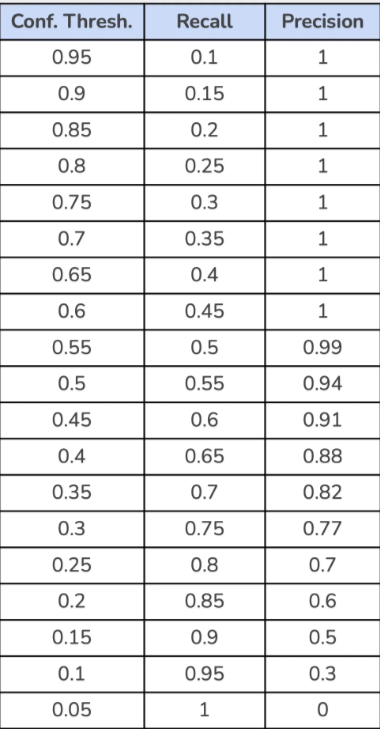
\includegraphics[width=0.35\linewidth]{tabd.png}
    \caption{Precision i Recall dla różnych wartości progu pewności detekcji}
    \label{fig:not}
\end{figure}
\FloatBarrier

\begin{figure}[h]
    \centering
    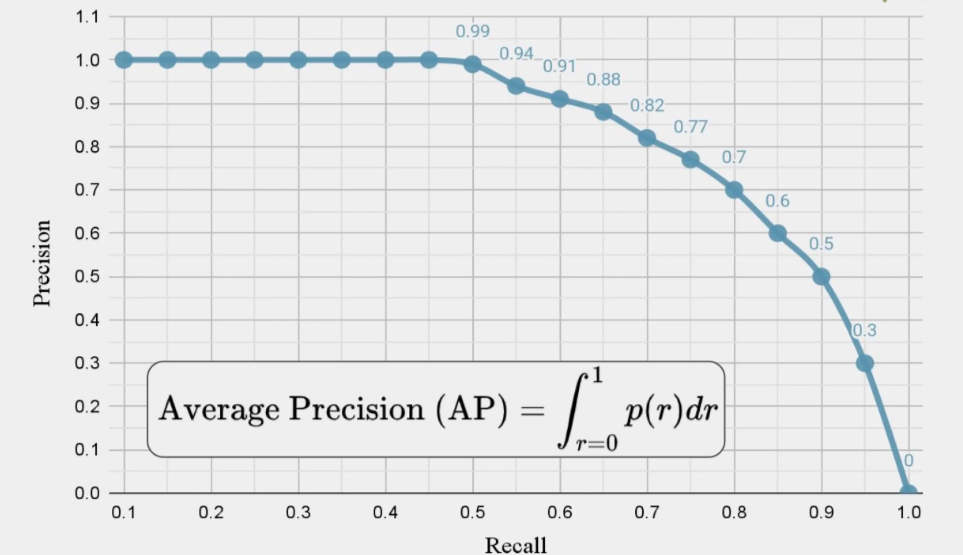
\includegraphics[width=0.58\linewidth]{Curveled.png}
    \caption{Krzywa precision-recall}
    \label{fig:good}
\end{figure}

\begin{defi}\label{map}
\emph{Mean Average Precision} (mAP) to średnia wartość Average Precision obliczona dla wszystkich klas w zbiorze danych. Ocenia ona ogólną skuteczność modelu detekcji obiektów.

Dwie najczęściej stosowane warianty tej metryki to:
\begin{itemize}
\item $mAP_{50}$ - średnia precyzja obliczona dla progu IoU równego 0.5,
\item $mAP_{50-95}$ - uśredniona wartość precyzji dla progów IoU od 0.5 do 0.95.
\end{itemize}
\end{defi}

\chapter{Zbiory danych}\label{Zbiory}

\section{TACO}

TACO to otwarty zbiór składający się z 1500 zdjęć zawierających 4784 instancji śmieci. Adnotacje zdjęć, zapisane w formacie COCO, pozwalają na użycie tego zbioru do treningu modeli do segmentacji lub detekcji. Co ważne zdjęcia zostały wykonane w przyrodzie, co jest dobrym odwzorowaniem sytuacji jakie nasz docelowy model będzie przetwarzał. Odpady przyporządkowane są do 60 kategorii oraz 28 super kategorii. Adnotacje oprócz klasyfikacji obiektów zawierają również etykiety dotyczące tła (“piasek”, “roślinność”). Trzecią najliczniejszą kategorią występującą w zbiorze są “śmieci nieoznaczone”. Kategoria ta obejmuje obiekty, które można zidentyfikować jako śmieci, jednak ich dokładna klasyfikacja jest utrudniona. Ze względu na dużą liczebność tej grupy, stanowi ona duże utrudnienie w kontekście realizacji naszego zadania.

\section{TrashBox}

TrashBox to otwarty zbiór danych, zawierający 17 785 zdjęć, stworzony przede wszystkim z myślą o klasyfikacji odpadów. Jest to jeden z największych datasetów w tej dziedzinie. Zbiór obejmuje kategorie, które rzadko pojawiają się w innych zbiorach danych, takie jak odpady elektroniczne oraz odpady medyczne.  

Obrazy w zbiorze zostały podzielone na 7 głównych klas:  
\begin{itemize}
    \item \textbf{Cardboard} – kartony i opakowania tekturowe (2 414 zdjęć),
    \item \textbf{E-waste} – odpady elektroniczne, takie jak smartfony, laptopy, przewody itp. (2 883 zdjęć),
    \item \textbf{Glass} – szklane przedmioty (2 528 zdjęć),
    \item \textbf{Medical waste} – odpady medyczne, w tym strzykawki, maski chirurgiczne i rękawiczki (2 010 zdjęć),
    \item \textbf{Metal} – przedmioty metalowe, takie jak puszki, złom konstrukcyjny, pojemniki (2 586 zdjęć),
    \item \textbf{Plastic} – różne formy plastiku, m.in. butelki, torby, pojemniki i niedopałki papierosów (2 669 zdjęć),
    \item \textbf{Paper} – gazety, kubki papierowe, opakowania (2 695 zdjęć).
\end{itemize}

Łącznie zbiór TrashBox zawiera 26 podkategorii, które stanowią bardziej szczegółowy podział w obrębie siedmiu głównych klas. Dzięki temu możliwe jest dokładniejsze rozróżnianie różnych typów odpadów, co zwiększa wartość tego zbioru jako zestawu treningowego.   

Zdjęcia w zbiorze TrashBox mają różne rozdzielczości, ale niewiele z nich przekracza 800 × 800 pikseli. Zbiór wyróżnia się tym, że zawiera zdjęcia odpadów w różnorodnych środowiskach, co znacznie odróżnia go innch zbiorów, które zazwyczaj zawierają jedynie zdjęcia na białym tle. Zdaniem autorów tego datasetu, zbiór TrashBox jest dobrym uzupełnieniem zbioru TACO, który nie zawiera wystarczającej liczby zdjęć.

\section{MS COCO}

Zbiór danych MS COCO (Microsoft Common Objects in Context) to jeden z najczęściej wykorzystywanych zestawów obrazów w zadaniach związanych z uczeniem maszynowym, zwłaszcza w kontekście rozpoznawania i segmentacji obiektów. Stanowi on wszechstronne źródło danych, pozwalające na trenowanie oraz ewaluację modeli w zakresie detekcji obiektów, segmentacji semantycznej i instancyjnej, analizy punktów kluczowych, a także generowania opisów tekstowych dla obrazów.  

Zbiór MS COCO zawiera 328 000 obrazów z 2,5 milionami oznaczonych instancji obiektów należących do 91 kategorii. W porównaniu do innych popularnych zbiorów, takich jak ImageNet czy PASCAL VOC, MS COCO wyróżnia się większą liczbą instancji na kategorię oraz większą liczbą obiektów na obraz. Zbiór MS COCO zawiera katerorię z różnych dziedzin życia, a nie tylko zdjęcia odpadów. Znajdziemy tu zdjęcia zarówno ludzi, zwierząt jak i przedmiotów codziennego użytku.

MS COCO stał się standardem w dziedzinie detekcji i segmentacji, a modele trenowane na tym zbiorze są szeroko wykorzystywane w badaniach i aplikacjach przemysłowych. Modele, które wykorzystaliśmy w naszych eksperymentach, były wstępnie trenowane na MS COCO, co pozwoliło im na skuteczniejsze rozpoznawanie struktury i cech obiektów.  

\chapter{Mask R-CNN}\label{MASKRCNN}

\section{Wybór Mask R-CNN}

Mask R-CNN to sieć neuronowa służąca do segmentacji obiektów na obrazach. Model wykrywa wszystkie obiekty widoczne na zdjęciu za pomocą nakładania na nie ramek, klasyfikuje je oraz pokrywa maskami. Naszym głównym celem jest uzyskanie modelu zdolnego do detekcji, jednak postanowiliśmy, iż warto przetestować działanie Mask R-CNN. Segmentacja nie jest dla nas konieczna, lecz jeśli wyniki byłyby zadowalające rozważylibyśmy rozszerzenie funkcjonalności naszego rozwiązania.

Poza tym Mask R-CNN to szybki (potrafi działać w zadowalający sposób z prędkością 5 fps) oraz prosty model pod względem architektury. Ponadto biblioteka torchvision zawiera metody pozwalające na załadowanie modelu i opcjonalne załadowanie wag tego modelu przetrenowanego wcześniej na jakimś zbiorze danych. W przypadku Mask R-CNN użyliśmy funkcji $maskrcnn\_resnet50\_fpn()$ oraz wag uzyskanych w wyniki treningu na zbiorze MS COCO. Funkcja ta pozwoli na zdecydowanie łatwiejszą implementację treningu, a wagi powinny sprawić, iż model bazowo będzie w stanie wykrywać wszystkie obiekty na zdjęciu.

\section{Opis Mask R-CNN}

\subsection{Ogólna architektura}

Mask R-CNN powstał jako rozszerzenie Faster R-CNN, które służy do detekcji oraz klasyfikacji obiektów. W związku z tym jego architektura jest podobna do swojego poprzednika. Najważniejszą różnicą jest dodatkowa głowa sieci służąca do segmentacji obiektów. Mask R-CNN składa się z dwóch głownych części: Region Proposal Network (RPN) oraz głów sieci.

\subsection{Backbone}
Sieć bazowa (backbone) służy do wydobycia cech z danych wejściowych. Do realizacji tego zadania autorzy Mask R-CNN wykorzystywali sieci takie jak ResNet, czy Feature Pyramid Network (FPN).

\subsection{Region Proposal Network}

Region Proposal Network to sieć neuronowa służąca do generowania regionów (RoI - Region of Interest) w których potencjalnie mogą znajdować się obiekty do wykrycia. Działa na podstawie cech ekstraktowanych przez backbone.

\subsection{RoIAlign}
RoIAlign to operacja służąca do wyodrębniania cech z regionów zainteresowania. Względem Faster R-CNN zastępuje ona operację RoIPool. Atutem RoIAlign jest to, że zachowuje dokładne współrzędne regionów zainteresowania, co jest kluczowe w kontekście zadania segmentacji.

\subsection{Głowy sieci}
Każdy przetworzony region zainteresowania trafia do trzech równoległych głów:

\begin{itemize}
    \item Klasyfikacja obiektów - odpowiada za przypisanie klasy do danego obiektu
    \item Regresja współrzędnych ramki (bounding box) - dopasowuje ramkę określającą położenie obiektu
    \item Segmentacja maski - nakłada binarną maskę na region zainteresowania 
\end{itemize}

\subsection{Funkcja straty}
Jako funkcję straty Mask R-CNN minimalizuje:
$$L=L_{cls}+L_{box}+L_{mask}$$

\begin{itemize}
    \item $L_{cls}$ - strata klasyfikacji
    \item $L_{box}$ - strata regresji ramki
    \item $L_{mask}$ - strata segmentacji maski
\end{itemize}

\section{Wyniki na zbiorze MS COCO}

Na początek oceniliśmy działanie przetrenowanego modelu MASK R-CNN na zbiorze walidacyjnym COCO. Zbiór ten liczy ponad 5000 zdjęć. Taki eksperyment miał służyć jako punkt odniesienia przed dalszym treningiem. Poniżej przedstawiamy wyniki eksperymentu:

\begin{itemize}
    \item Precision (Precyzja): $17.23\%$
    \item Recall (Czułość): $79.69\%$
    \item $mAP_{50}$: $58.17\%$
    \item $mAP_{50-95}$: $37.27\%$
\end{itemize}



Te wyniki pokazują, że model radzi sobie dobrze pod względem wykrywalności obiektów, ale wśród wszystkich generowanych predykcji tylko nieznaczna część jest poprawna, zatem model generuje sporo fałszywych pozytywów. Po zwizualizowaniu wygenerowanych obiektów na obrazkach zauważyliśmy, że model ma tendencję do generowania zbyt dużej liczby ramek. Wiele z generowanych ramek nakładało się na siebie.

\section{Pierwsze eksperymenty}
\subsection{Implementacja treningu}
Do implementacji treningu Mask R-CNN na zbiorze TACO użyliśmy biblioteki torchvision, która udostępnia funkcję maskrcnn\_resnet50\_fpn(), która ładuje model wraz z wagami dostępnymi poprzez parametr MaskRCNN\_ResNet50\_FPN\_Weights.COCO\_V1.


\begin{verbatim}
    model = torchvision.models.detection.maskrcnn_resnet50_fpn(weights=
    torchvision.models.detection.MaskRCNN_ResNet50_FPN_Weights.DEFAULT)

\end{verbatim}
W pierwszych eksperymentach będziemy trenować jedynie ostatnie warstwy odpowiedzialne za predykcję ramek i masek. Pozostałe parametry zamroziliśmy, aby podczas treningu nie zmieniały swoich wartości. Decyzja ta wynika z tego, iż jak na razie dysponujemy małym zbiorem danych, a aby skutecznie wytrenować cały model potrzeba by było zdecydowanie większej ilości zdjęć. Poza tym Mask R-CNN przez to, że jest już pretrenowany na zbiorze MS COCO powinien radzić sobie z nakładaniem ramek i segmentacją obiektów, a co za tym idzie możliwe że nie ma potrzeby treningu wszystkich warstw. %Mimo to przeprowadzimy również eksperymenty z treningiem większej ilości warstw.

\begin{verbatim}
    for param in model.parameters():
        param.requires_grad = False
        
    model.roi_heads.box_predictor = torchvision.models.detection.faster_rcnn.
    FastRCNNPredictor(in_channels=1024, num_classes=num_classes)
    
    model.roi_heads.mask_predictor = torchvision.models.detection.mask_rcnn.
    MaskRCNNPredictor(in_channels=256, dim_reduced=256, num_classes=num_classes)
\end{verbatim}
\subsection{Pierwszy trening}
Zbiór treningowy składał się z 1200 zdjęć ze zbioru TACO. Zbiór walidacyjny i testowy zawierały po 150 zdjęć z tego zbioru. Wszystkie eksperymenty modelu Mask R-CNN były przeprowadzane na tym zbiorze testowym. Klasyfikacja obiektów odbywała się na 60 klasach - domyślnych kategorii w zbiorze TACO.
Jako optymalizatora użyliśmy SGD z biblioteki torch.
\begin{verbatim}
    optimizer = torch.optim.SGD(
        model.parameters(), lr=0.001, momentum=0.9, weight_decay=0.0005
    )
\end{verbatim}


Wyniki prezentują się następująco:


\begin{itemize}
    \item Precision (Precyzja): $5\%$
    \item Recall (Czułość): $44\%$
    \item $mAP_{50}$: $22.4\%$
    \item $mAP_{50-95}$: $17\%$
\end{itemize}

Wyniki, zgodnie z tym czego się spodziewaliśmy są niezadowalające. Jedną z przyczyn takiego wyniku jest liczba klas. Osiągnięcie zadowalających wyników dla 60 klas z tak małą ilością zdjęć nie jest możliwe. Ponadto rozkład obiektów ze względu na klasy jest bardzo nierówny.
\subsection{Klasy w zbiorze TACO}

W zbiorze TACO, śmieci są przyporządkowywane do jednej z 60 kategorii. Do najliczniejszych klas należą, między innymi: papierosy, nieoznaczone śmieci, folia plastkiowa i plastikowe butelki. Klasy jednak są niezbalansowane i kilka najliczniejszych klas dominuje całą resztę. W związku z tym model wytrenowany na takich kategoriach będzie miał tylko szanse dobrze klasyfikować obiekty należące do tych największych klas. 



Zbiór TACO posiada także przyporządkowanie obiektów do jednej z 28 superkategorii. Są to ogólniejsze klasy, które łączą w sobie część podstawowych klas, przykładowo superkategoria "Słomki"\ zawiera w sobie obiekty opisane jako "Słomki plastikowe"\ oraz "Słomki papierowe". Rozwiązenie to zmniejsza ilość klas dzięki czemu rozkład ilości obiektów nie jest już tak nierówny co w podstawowych klasach (nadal jednak kilka klas dominuje resztę, a kilka ma niewiele reprezentantów w zbiorze). Niestety użycie superkategorii w naszym treningu jest niemożliwe, gdyż klasy nie są grupowane po materiale odpadu (przykład ze słomkami). 


Z tego powodu postanowiliśmy stworzyć własne mapowanie klas zbioru TACO. Grupowaliśmy śmieci przede wszystkim po materiale z jakiego są wykonane oraz po ich ogólnym przeznaczeniu. Przykładowo jedną z nowych klas była klasa "Karton", do której należały między innymi klasy: "Karton po pizzy", "Karton po jajkach", "Inny karton". W ten sposób uzyskaliśmy 36 klas. Rozkład ilości obiektów nadal jest nierówny, natomiast bardziej zrównoważony niż w orginalnych 60 klasach.

\subsection{Eksperyment z nowym mapowaniem klas}

W kodzie implementującym trening jedynymi zmianami była inna liczba klas oraz dodanie mapowania kategorii ze zbioru TACO na nasze kategorie.
\\

Wyniki eksperymentu wynoszą:

\begin{itemize}
    \item Precision (Precyzja): $5.4\%$
    \item Recall (Czułość): $47\%$
    \item $mAP_{50}$: $23\%$
    \item $mAP_{50-95}$: $17.4\%$
\end{itemize}

Wyniki dla tego eksperymentu były minimalnie lepsze w porównaniu do poprzedniego eksperymentu, jednak nadal niezadowalające. Problemem nadal z pewnością była liczba klas oraz ich niezbalansowanie, natomiast zdawaliśmy sobie sprawę, że do osiągnięcia zadowalających rezultatów będzie potrzeba większego zbioru danych, a więc postanowiliśmy się przyjrzeć innym otwartym zbiorom danych śmieci.

\subsection{Przygotowanie zbioru TrashBox} 
Do powiększenia naszego zbioru danych postanowiliśmy skorzystać ze zbioru TrashBox. Zbiór ten jednak służy do klasyfikacji obiektów, dlatego przed użyciem musieliśmy przygotować własnoręcznie odpowiednie adnotacje. W tym celu użyliśmy narzędzia Make Sense, które umożliwia wczytanie zdjęć, narysowanie masek oraz przyporządkowanie odpowiedniej klasy do obiektu. Po zakończeniu tworzenia adnotacji można je eksportować do formatu COCO.

\subsection{Treningi ze zbiorem TrashBox}
Pierwszym eksperymentem który przeprowadziliśmy był trening jedynie na zbiorze TrashBox. Chcieliśmy w ten sposób sprawdzić, czy uzyskane przez nas do tej pory zdjęcia i adnotacje mają szansę poprawić wcześniejsze wyniki. W stowrzonym przez nas zbiorze znalazło się 1513 zdjęć z obiektami przyporządkowanymi do 14 klas. Część kategorii z oryginalnego zbioru TrashBox postanowiliśmy odrzucić z powodu małej ilości reprezentowanych obiektów. Wyniki eksperymentu wyniosły:

\begin{itemize}
    \item Precision (Precyzja): $4\%$
    \item Recall (Czułość): $30\%$
    \item $mAP_{50}$: $8\%$
    \item $mAP_{50-95}$: $5\%$
\end{itemize}

Wyniki są bardzo niskie , natomiast przeprowadziliśmy również eksperyment na połączonych zbiorach TACO i TrashBox, aby móc porównać wprost wyniki nowego powiększonego zbioru i samego zbioru TrashBox. W tym celu wykonaliśmy mapowanie klas z TACO na klasy zbioru TrashBox. Tym samym w nowym zbiorze nie znalazły się już kategorie z TACO zawierające po kilka lub kilkanaście zdjęć, m. in. baterie, czy opakowania po pizzy. Wyniki prezentują się następująco:

\begin{itemize}
    \item Precision (Precyzja): $4.2\%$
    \item Recall (Czułość): $56\%$
    \item $mAP_{50}$: $17.9\%$
    \item $mAP_{50-95}$: $13.9\%$
\end{itemize}

Wyniki są lepsze niż dla samego zbioru TrashBox, nadal jednak są na tyle niskie, że oczywistym wnioskiem stało się, iż nadal mamy za mało zdjęć jak na taką liczbę klas. Z tego powodu postanowiliśmy skorzystać z podziału na główne klasy, jaki znajduje się w zbiorze TrashBox. Z siedmiu kategorii wybraliśmy ostatecznie pięć (Cardboard, Glass, Metal, Plastic, Paper), a odrzuciliśmy kategorie E-waste i Medical waste. Wynikało to przede wszystkim z niewielkiego pokrycia tych kategorii jeśli chodzi o sam zbiór TrashBox, ale także TACO. 
Kolejny eksperyment przeprowadziliśmy zatem dla połączonego zbioru TACO i TrashBox na pięciu klasach obiektów. Otrzymane wyniki to:

\begin{itemize}
    \item Precision (Precyzja): $6.4\%$
    \item Recall (Czułość): $64.7\%$
    \item $mAP_{50}$: $30\%$
    \item $mAP_{50-95}$: $22.2\%$
\end{itemize}

Co było oczekiwane wyniki są wyższe, natomiast aby osądzić, czy zbiór TrashBox rzeczywiście poprawia wyniki przeprowadziliśmy ten sam eksperyment, ale na samym zbiorze TACO. Wyniki były następujące:

\begin{itemize}
    \item Precision (Precyzja): $6\%$
    \item Recall (Czułość): $76\%$
    \item $mAP_{50}$: $45\%$
    \item $mAP_{50-95}$: $33\%$
\end{itemize}

A zatem wyniki (poza precyzją) są zauważalnie wyższe dla treningu na samym zbiorze TACO. Wynikało to według nas ze specyfiki zbioru TrashBox. Przede wszytskim zbiór ten powstał do zadania klasyfikacji i nawet mimo tego, że stworzyliśmy sami adnotacje potrzebne do segmentacji, zdjęcia nadal nie były do tego optymalnie przystosowane. Każde zdjęcie zawierało tylko jedną klasę obiektów, a ponadto znacznie różniły się one od zdjęć w zbiorze TACO. Obiekty w TrashBox często zajmowały znaczną część zdjęcia i były umiejscowione centralnie. Część obiektów znajdowała się na białym tle, co jest nierealistyczne w kontekście naszego zastosowania. Kolejnym czynnikiem, który mógł sprawić, że wyniki się pogorszyły było to, że większość zdjęć w zbiorze TrashBox jest małej rozdzielczości.

Z tego powodu w następnych eksperymentach wróciliśmy do treningów na samym zbiorze TACO. Mimo to rozmiar zbioru danych nadal był problemem, dlatego rozpoczeliśmy w międzyczasie pracę nad własnym zbiorem danych.

\section {NMS i Próg pewności detekcji}

\subsection{NMS}
Jako, że celem zadania detekcji obiektów jest wygenerowanie dokładnie jednej detekcji na obiekt, powszechną praktyką jest założenie, że silnie nakładające się detekcje należą do tego samego obiektu i należy je połączyć w jedną detekcję. W tym celu stosuję się technikę Non-maximum supperssion.

\textbf{Non-maximum suppression (NMS)} to algorytm stosowany w wykrywaniu obiektów w celu eliminacji nadmiarowych detekcji, które w znacznym stopniu pokrywają się z detekcjami o wyższym poziomie pewności. Technikę Non-Maximum Suppression można stosować przy różnych progach IoU. Parametr ten określa stopień nakładania się ramek ograniczających, powyżej którego mniej pewne detekcje są usuwane. Niższa wartość IoU oznacza, że NMS będzie bardziej agresywnie eliminować nakładające się ramki, podczas gdy wyższa wartość pozwala na zachowanie większej liczby detekcji.
Poniżej przedstawiamy przykład użycia NMS:

\begin{figure}[h]
    \centering
    \begin{minipage}{0.45\textwidth}
        \centering
        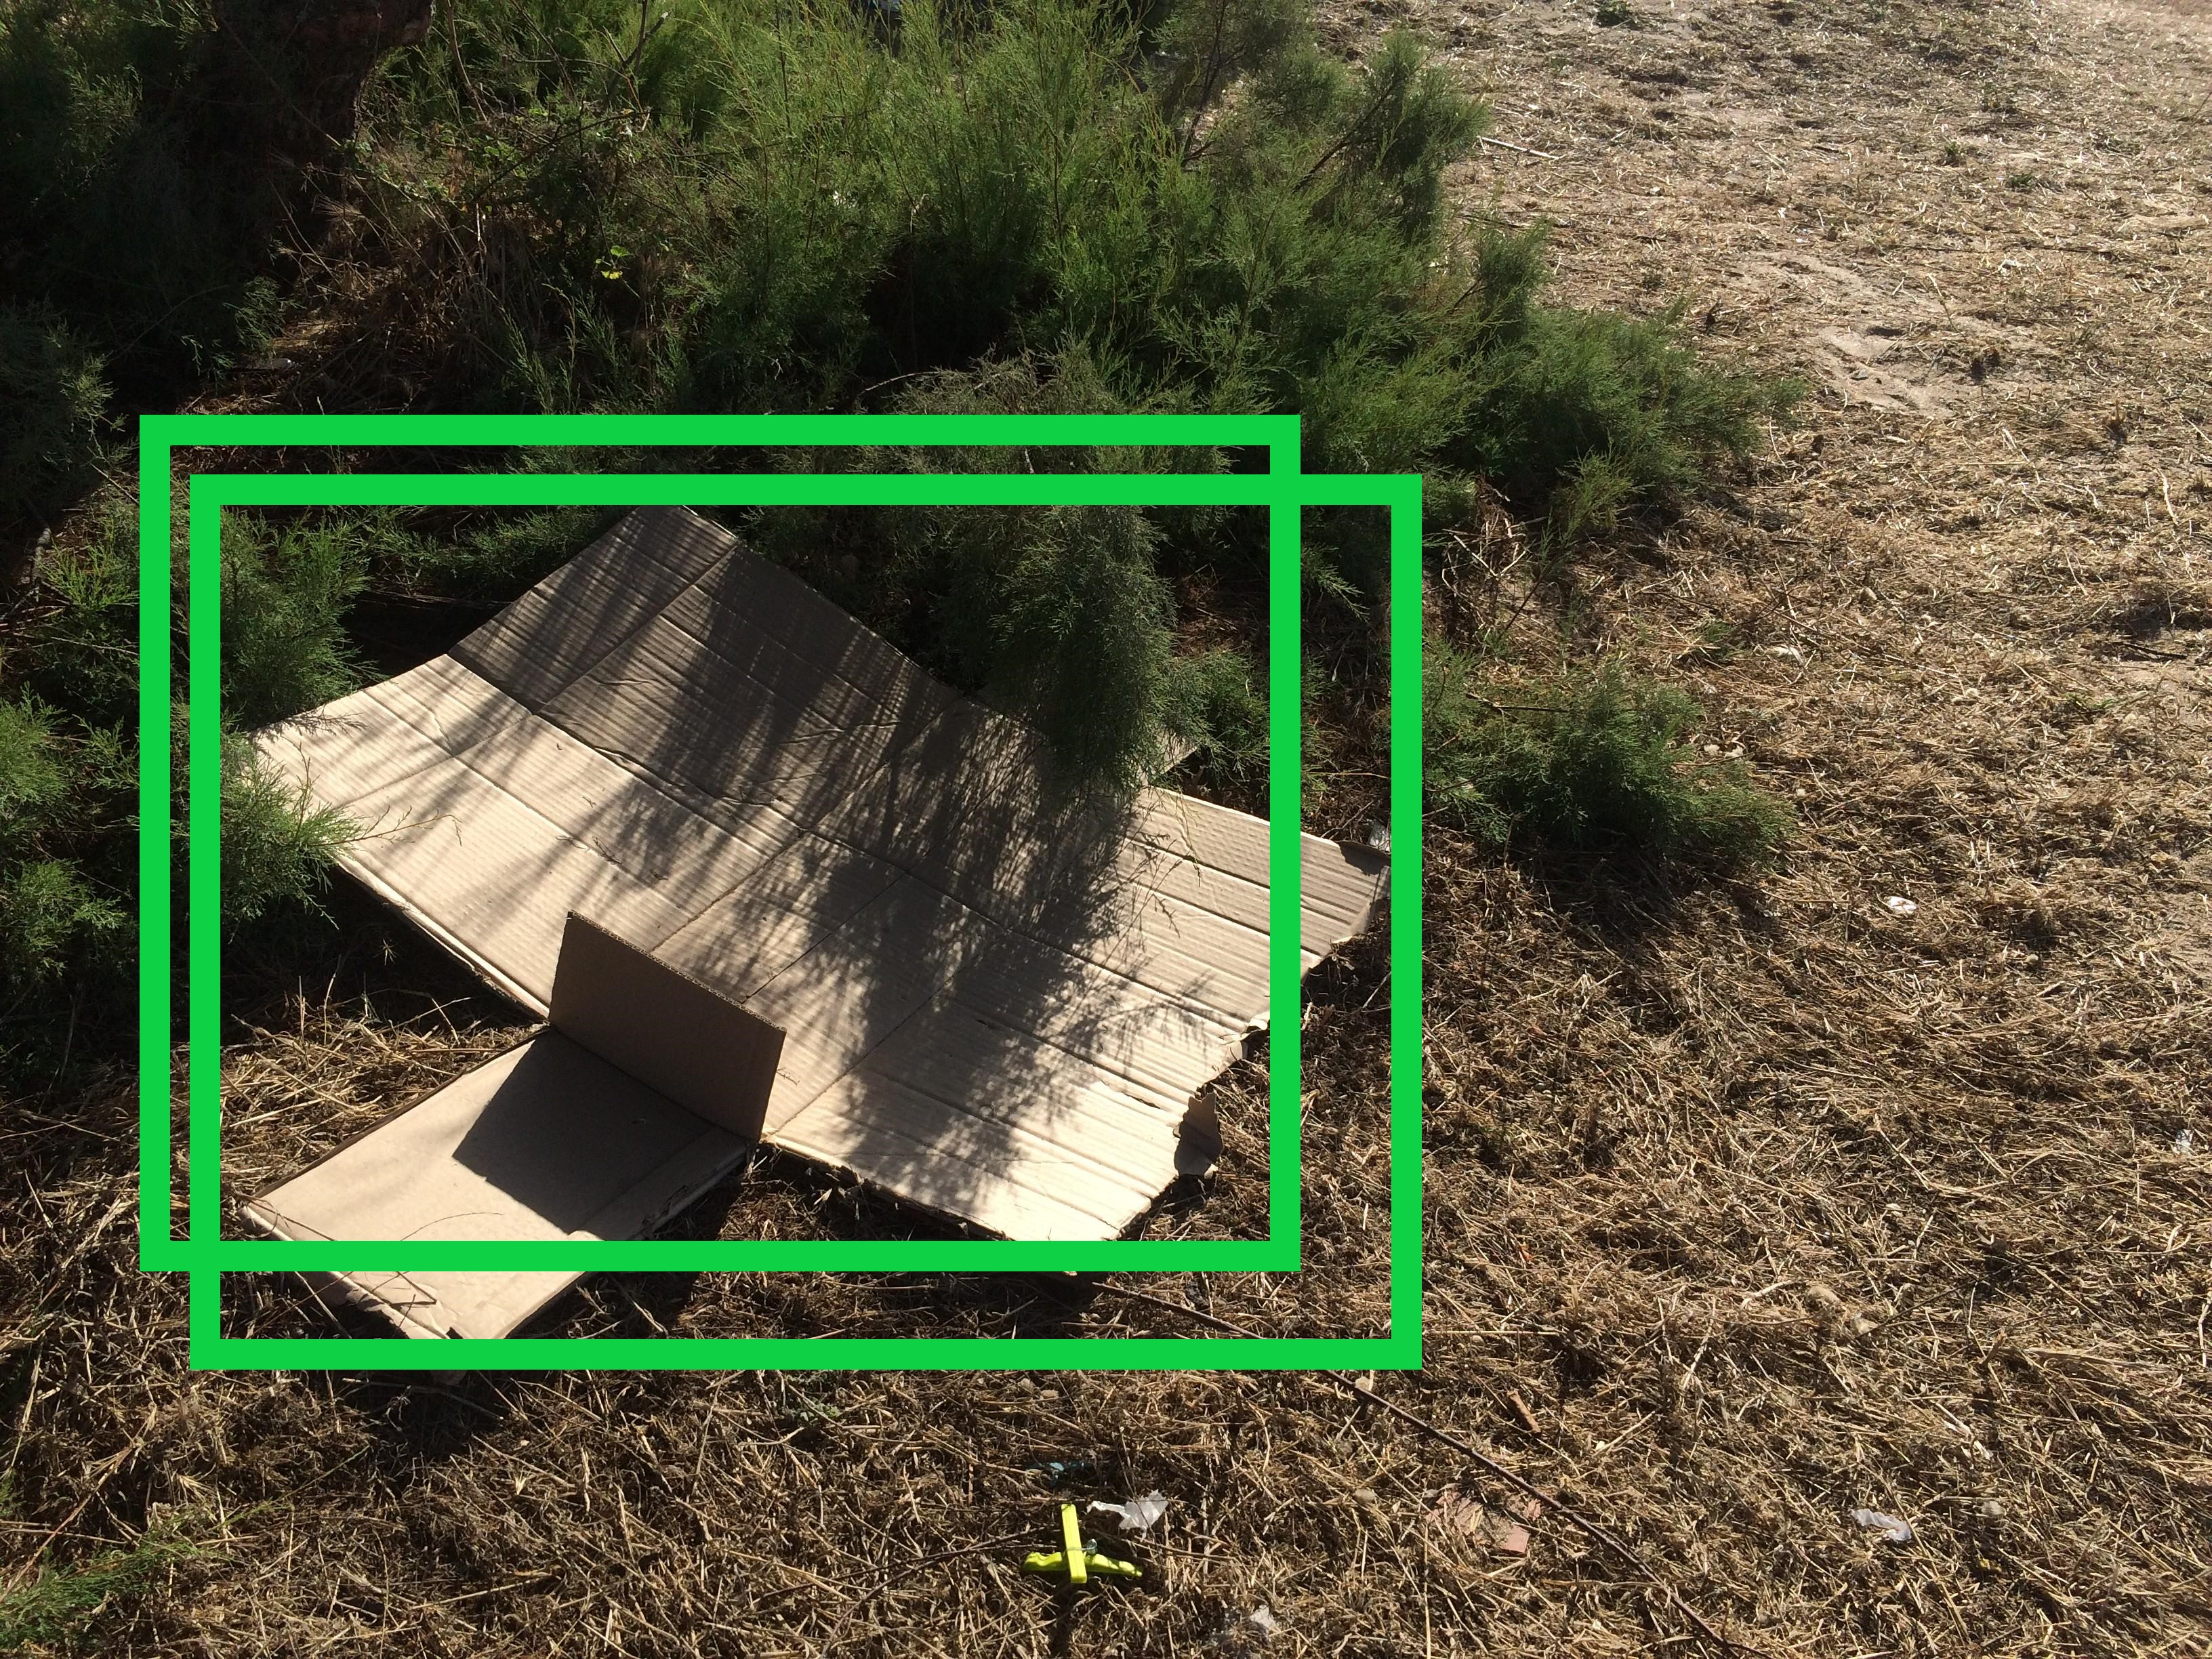
\includegraphics[width=\linewidth]{not000050.jpg}
        \caption{Przed użyciem NMS}
        \label{fig:not}
    \end{minipage}
    \hfill
    \begin{minipage}{0.45\textwidth}
        \centering
        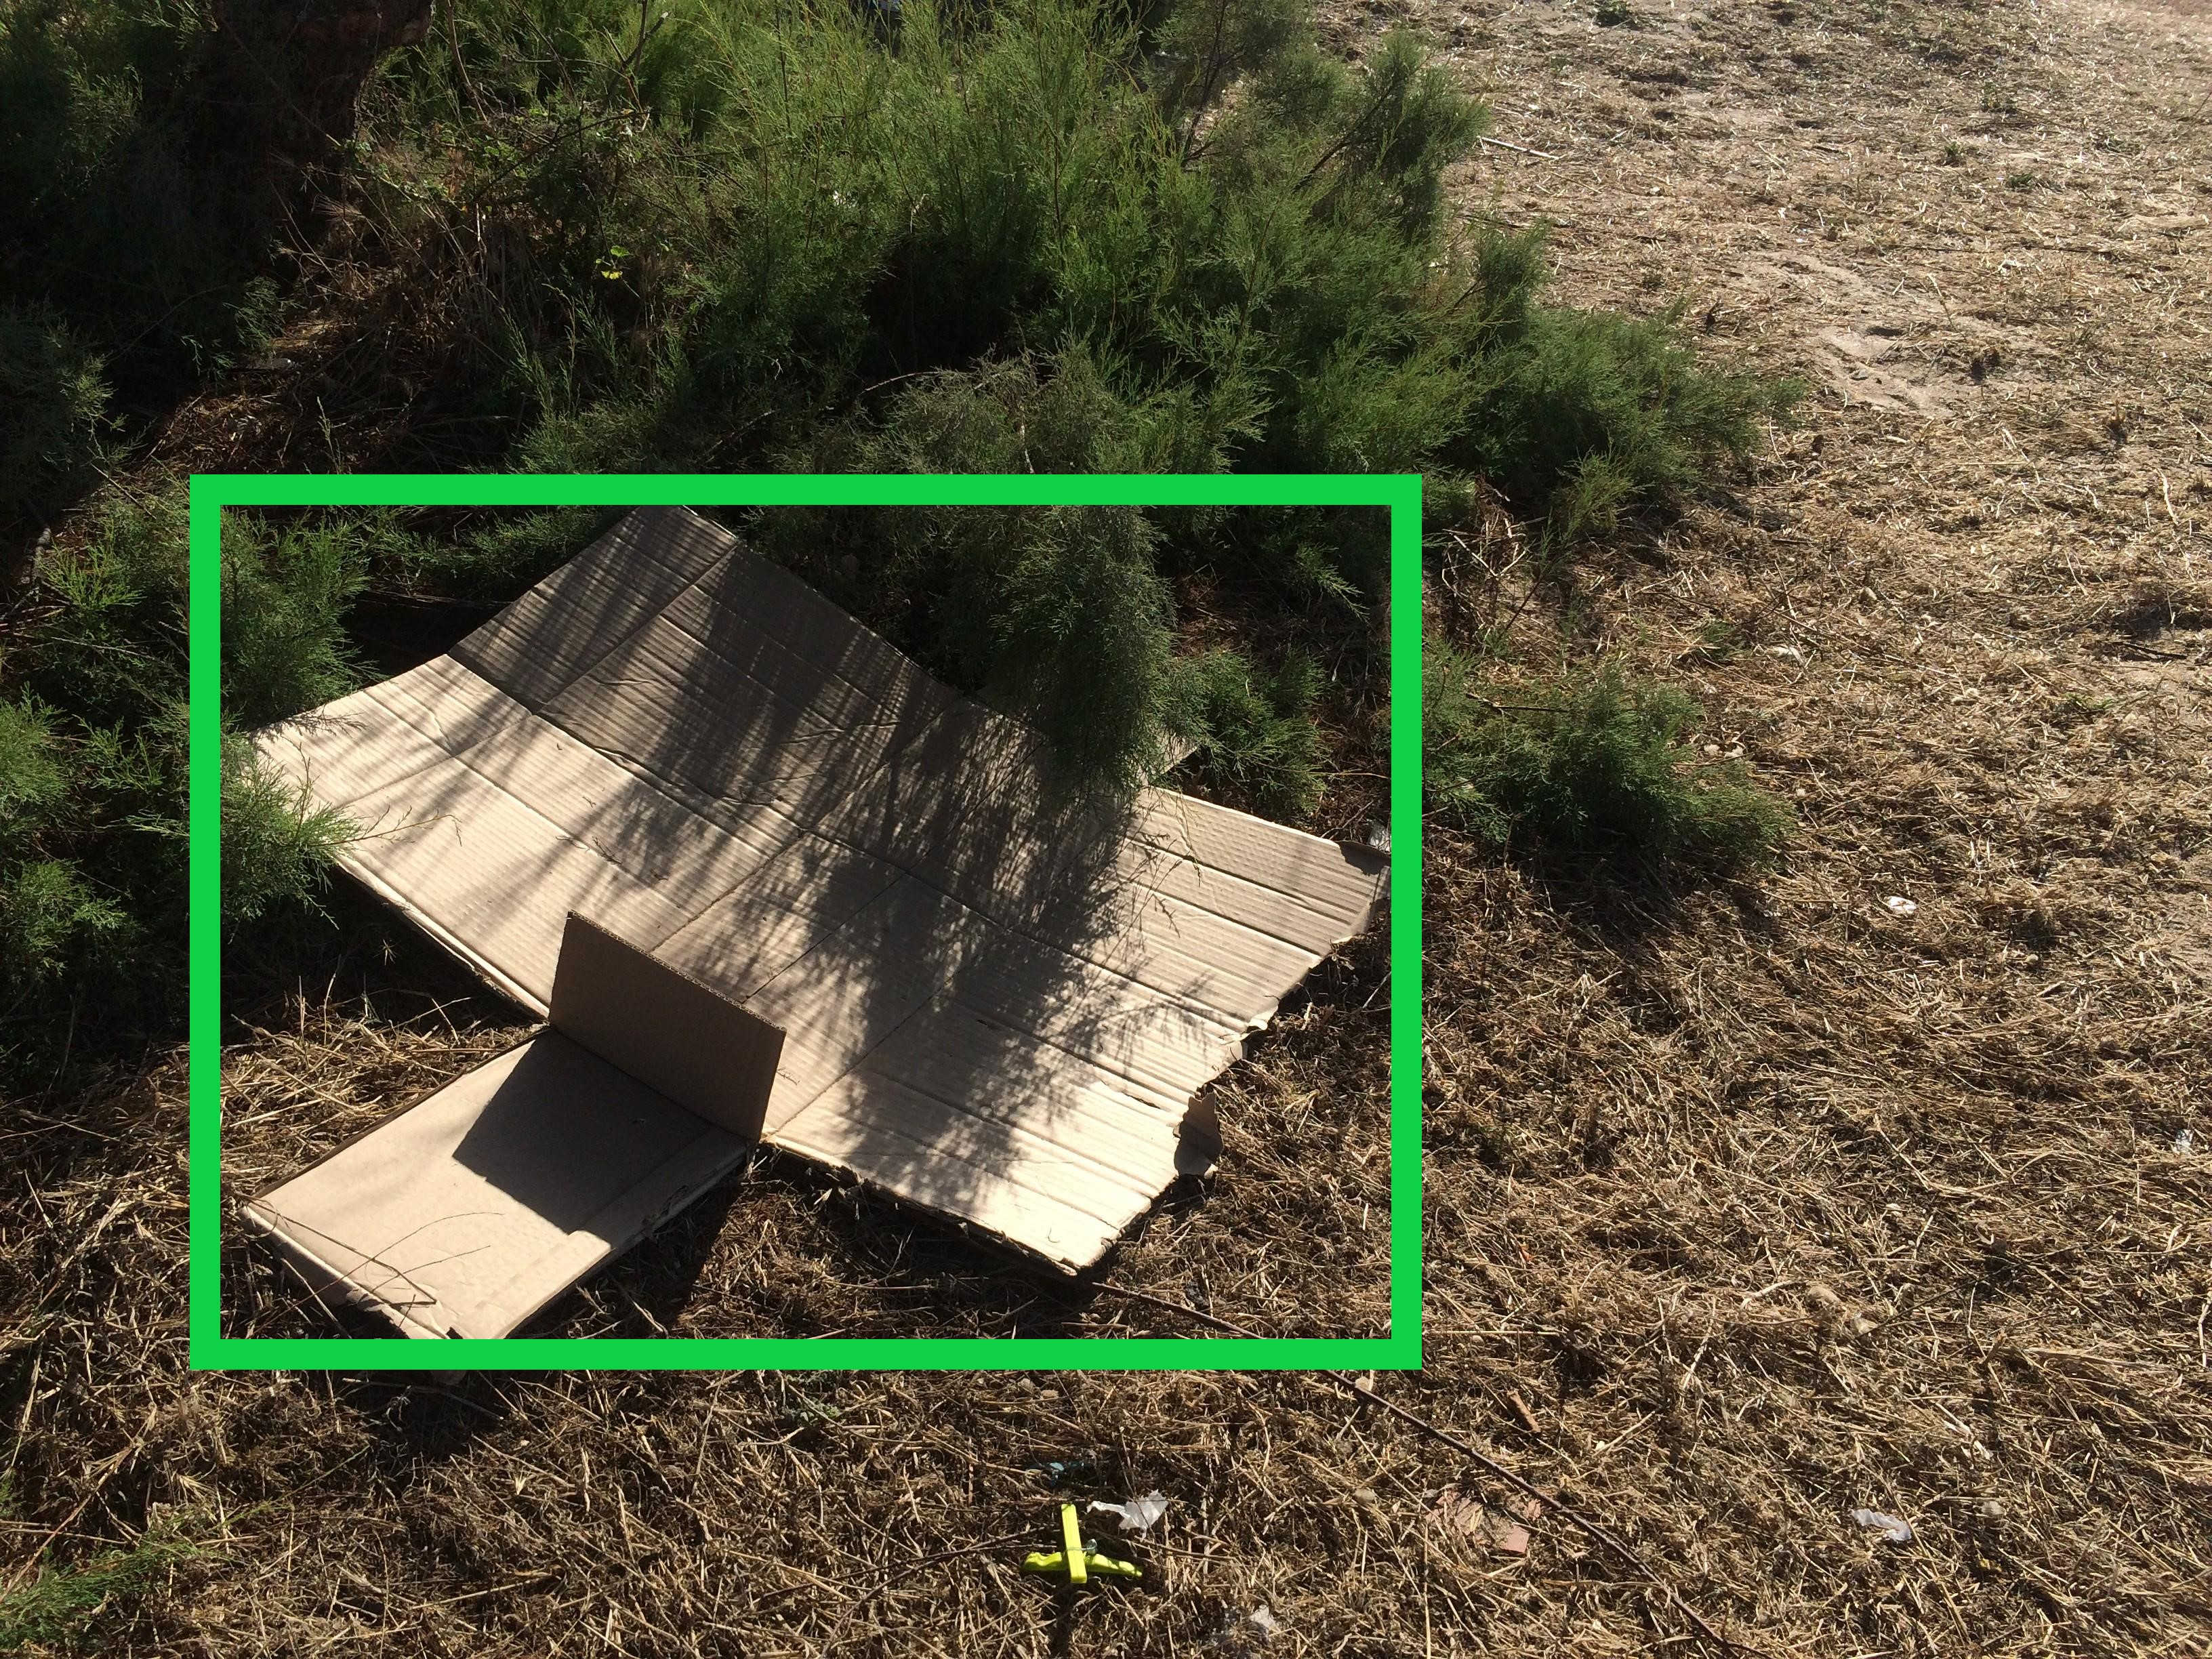
\includegraphics[width=\linewidth]{good000050.jpg}
        \caption{Po użyciu NMS}
        \label{fig:good}
    \end{minipage}
    \caption{Przykład użycia NMS}
\end{figure}

\subsection{Próg pewności detekcji}
Model Mask R-CNN przy okazji każdej wygenerowanej predykcji zwraca również prawdopodobieństwo danej detekcji.  Predykcje o niskim poziomie pewności często są błędne lub nieprecyzyjne. Dlatego też dobrym pomysłem w zdaniach detekcji często okazuje się zachowanie tylko tych detekcji, które są najbardziej wiarygodne. Żeby tego dokonać kluczowe jest ustawiene progu pewności detekcji.

\subsection{Analiza problemu nakładających się detekcji}
Podczas eksperymentów z modelem Mask R-CNN zaobserwowaliśmy tendencję do generowania dużej liczby nakładających się ramek. Model często wykrywał ten sam obiekt wielokrotnie, co prowadziło do dużych wartości recall kosztem bardzo niskiego poziomu precision.

Aby zredukować efekt nakładających się ramek oraz zmniejszyć liczbę generowanych predykcji, zastosowaliśmy techniki Non-Maximum Suppression  oraz dostosowanie progu pewności detekcji.   

\subsection{Wyniki}

W tabeli poniżej przedstawiamy wpływ wyżej wymienionych technik na wskaźniki jakości detekcji.  

\begin{table}[h]
    \centering
    \caption{Wpływ NMS i progu pewności na jakość detekcji}
    \label{tab:nms_results}
    \begin{tabular}{|c|c|c|c|c|c|c|}
        \hline
        \textbf{NMS} & \textbf{IoU} & \textbf{Próg pewności} & \textbf{Precision} & \textbf{Recall} & \textbf{mAP$_{50}$} & \textbf{mAP$_{50-95}$} \\
        \hline
        Nie & - & 0.0 & 6.0\% & 76.0\% & 45.0\% & 33.0\% \\
        Nie & - & 0.4 & 32.8\% & 55.8\% & 34.7\% & 26.5\% \\
        Nie & - & 0.55 & 45.0\% & 46.0\% & 30.9\% & 23.6\% \\
        Nie & - & 0.6 & 50.2\% & 40.9\% & 28.0\% & 21.4\% \\
        Tak & 0.25 & 0.0 & 9.0\% & 58.6\% & 31.8\% & 23.7\% \\
        Tak & 0.25 & 0.3 & 28.7\% & 50.7\% & 31.3\% & 23.5\% \\
        Tak & 0.5 & 0.3 & 26.2\% & 53.5\% & 31.8\% & 23.8\% \\
        Tak & 0.5 & 0.5 & 41.6\% & 50.0\% & 31.8\% & 24.2\% \\  
        Tak & 0.5 & 0.55 & 45.3\% & 45.9\% & 31.0\% & 23.8\% \\
        \hline
    \end{tabular}
\end{table}

\subsection{Wnioski}
Zastosowanie NMS miało tylko nieznaczny wpływ na poprawę wskaźników jakości detekcji. Wprowadzenie tej techniki doprowadziło do niewielkiego wzrostu precision, jednak odbyło się to kosztem recall.   

Znacznie większy wpływ na jakość detekcji miał próg pewności. Wartości w tabeli pokazują, że zwiększanie progu pewności prowadziło do wyraźnego wzrostu precision, ale jednocześnie skutkowało spadkiem recall. Dla niskiego progu (0.0) model wykrywał niemal wszystkie obiekty, osiągając recall na poziomie 76.0\%, jednak precyzja była bardzo niska (6.0\%), co oznaczało dużą liczbę fałszywych detekcji. Ostatecznie najlepsze wyniki model osiągnął dla progu pewności równym 0.55. 

Najbardziej zrównoważone wyniki osiągnięto dla \textbf{NMS z IoU = 0.50 oraz progu pewności 0.55}, gdzie uzyskano precision na poziomie 45.3\% oraz recall 45.9\%. W kolejnych eksperymentach będziemy stosować tę konfigurację jako domyślną, ponieważ zapewnia ona kompromis pomiędzy eliminacją fałszywych detekcji a zachowaniem wystarczającej liczby wykrytych obiektów.

\section{Treningi wielu warstw}
%Do tej pory wszystkie eksperymenty modyfikowały tylko
TODO

\section{Augmentacje}

Ze względu na ograniczoną liczbę obrazów w zbiorze danych, zdecydowaliśmy się na zastosowanie augmentacji danych. Augmentacja to technika sztucznego generowania nowych zdjęć w zbiorze treningowym na podstawie istniejących danych, poprzez stosowanie różnorodnych transformacji na obrazach. Pozwala to na zwiększenie odporności modelu na zmienność danych wejściowych oraz poprawę jego ogólnej skuteczności, a także może okazać się pomocne w zapobieganiu przeuczenia.  

W naszych eksperymentach augmentacje były stosowane dynamicznie, w trakcie treningu, co oznacza, że każdy obraz podlegał losowym przekształceniom przy każdym przejściu przez model. Dzięki takiemu zabiegowi model nie tylko trenował na oryginalnych obrazach, ale także na ich zmodyfikowanych wariantach.

Do przeprowadzania augmentacji wykorzystaliśmy bibliotekę Albumentations, która jest jedną z najszybszych i najpopularniejszych bibliotek do przetwarzania obrazów w języku Python. Dzięki wysokiej wydajności pozwala ona na efektywne rozszerzanie zbioru treningowego bez znaczącego wydłużenia czasu trenowania modelu.  

Zastosowane augmentacje można podzielić na kilka kategorii:  

\begin{itemize}
    \item \textbf{Losowy obrót o 90 stopni} – obraca obraz o 90 stopni. Pomaga modelowi w rozpoznawaniu obiektów niezależnie od ich orientacji.
    \item \textbf{Szum gaussowski} – nakłada na obraz losowy szum o różnym natężeniu. Zwiększa odporność modelu na zakłócenia, które mogą występować w rzeczywistych danych.
    \item \textbf{Rozmycie} – stosuje efekt rozmazania przypominający ruch
    \item \textbf{Odbicie w poziomie} – symetrycznie odbija obraz w poziomie. Pomaga modelowi nauczyć się rozpoznawania obiektów w różnych orientacjach.
    \item \textbf{Zmiana jasności i kontrastu} – losowo dostosowuje jasność i kontrast obrazu w określonym zakresie. Pozwala to modelowi lepiej radzić sobie z różnymi warunkami oświetleniowymi.
    \item \textbf{Modyfikacja barw} – zmienia odcień, nasycenie i wartość koloru obrazu w losowy sposób. Poprawia zdolność modelu do rozpoznawania obiektów w zróżnicowanych warunkach barwnych.
\end{itemize}

Wyniki, przy trenowaniu tylko ostatnich warstw:

\begin{itemize}
    \item Precision (Precyzja): $43.2\%$
    \item Recall (Czułość): $38.5\%$
    \item $mAP_{50}$: $29.0\%$
    \item $mAP_{50-95}$: $23.2\%$
\end{itemize}

Uzyskane wyniki wskazują na pogorszenie skuteczności modelu po zastosowaniu augmentacji. Precyzja spadła do 43.2\% (z 45.3\%), a czułość do 38.5\% (z 45.9\%), co oznacza, że model częściej generował błędne detekcje i pomijał więcej obiektów. Może to sugerować, że zastosowane przekształcenia były zbyt agresywne lub nieodpowiednie dla dostępnego zbioru danych, co wpłynęło na gorszą zdolność modelu do generalizacji.

Przeprowadziliśmy również eksperyment, w którym sprawdzamy augmentacje przy trenowaniu większej liczby warstw. Wyniki prezentują się następująco:

\begin{itemize}
    \item Precision (Precyzja): $43.56\%$
    \item Recall (Czułość): $45.6\%$
    \item $mAP_{50}$: $31.6\%$
    \item $mAP_{50-95}$: $22.8\%$
\end{itemize}

Dzięki zastosowanym augmentacjom model miał możliwość nauki na bardziej zróżnicowanych danych, co pozwoliło mu lepiej radzić sobie z rzeczywistymi warunkami. Model uzyskał lepsze o kilka punktów procentowych wyniki niż jego odpowiednik bez stosowania augmentacji. Wyniki zbliżyły się do najlepszych dotychczas uzyskanych rezultatów.

\section{EfficientNet-Lite + Mask R-CNN}

W trakcie eksperymentów zaobserwowaliśmy, że model EfficientNet-Lite osiągał bardzo dobre wyniki na zbiorze TrashBox, skutecznie klasyfikując obiekty należące do 7 głownych kategorii oraz do 26 podkategorii (Treningi modelu EfficientNet-Lite zostały opisane w rozdziale X). Z kolei model Mask R-CNN lepiej wykrywał obszary zawierające śmieci, generując bardziej precyzyjne ramki, jednak miał większe trudności z poprawnym przypisaniem klasy do wykrytego obiektu.  

Na podstawie tych obserwacji zdecydowaliśmy się przeprowadzić eksperyment łączący obie architektury. Podejście to polegało na następujących krokach:
\begin{enumerate}
    \item Obraz wejściowy był przetwarzany przez Mask R-CNN, który generował ramki ograniczające dla wykrytych obiektów.
    \item Następnie wycinaliśmy fragmenty obrazu odpowiadające wykrytym ramkom.
    \item Każdy taki fragment był przekazywany do modelu EfficientNet-Lite, który miał za zadanie go sklasyfikować do odpowiedniej klasy
\end{enumerate}

Wyniki prezentują się następująco:

\begin{itemize}
    \item Precision (Precyzja): $28.9\%$
    \item Recall (Czułość): $33.5\%$
    \item $mAP_{50}$: $24.7\%$
    \item $mAP_{50-95}$: $19.2\%$
\end{itemize}

Niestety, uzyskane wyniki okazały się gorsze niż przy wykorzystaniu pojedynczych modeli. Przyczyną tego mogł być fakt, że zbiór TrashBox zawiera dobrą reprezentację 26 klas odpadów, lecz nie obejmuje wszystkich możliwych rodzajów śmieci. W rezultacie, model EfficientNet-Lite miał trudności z klasyfikacją obiektów spoza tych kategorii, co negatywnie wpłynęło na wyniki na zbiorze testowym TACO.  

Eksperyment ten pokazuje, że choć połączenie detekcji i klasyfikacji w osobnych modelach wydaje się intuicyjne, skuteczność takiego podejścia zależy w dużej mierze od reprezentatywności zbioru treningowego. W przyszłości warto rozważyć trenowanie klasyfikatora na bardziej zróżnicowanym zbiorze, aby poprawić zdolność modelu do generalizacji na nieznane obiekty.

\section{Wnioski}
TODO

\end{document}


%%% Local Variables:
%%% mode: latex
%%% TeX-master: t
%%% coding: latin-2
%%% End:
